\label{chap:kapitel3_3}
\section{Algorithmus von Reingold und Tilford}
Das Paper “Tidier Drawings of Trees” von Edward M. Reingold und John S. Tilford aus dem Jahre 1981,
welches im IEEE Transaction on Software Engineering erschienen ist, handelt von einem Algorithmus zum Zeichnen von Bäumen im Ebenen-Layout.
Die Motivation der beiden Autoren für das Erstellen dieses Algorithmus beruht darauf, dass sie ein entscheidendes Problem an dem 
verbesserten Algorithmus von Wetherell und Shannon erkannt haben. Dieser Algorithmus produziert, wie in Abschnitt XXX näher beschrieben, 
Bäume, welche nicht maximal schmal sind, da das Zentrieren der Väter erzwungen wird. Die modifizierte Variante des Algorithmus produziert 
zwar maximal schmale Bäume, dafür können diese wesentlich unübersichtlicher sein, was der untere Baum auf Abbildung XXX zeigt. 
Reingold und Tilford erkennen, dass das Problem an dem Algorithmus ist, dass die einzelnen Subtrees von Knoten außerhalb des Subtrees 
beeinflusst werden. Daraus folgern die beiden, dass es mit dem Algorithmus von Wetherell und Shannon dazu kommen kann, dass ein Baum und 
die Spiegelung desselben Baumes keine Spiegelbilder ergeben. Jedoch wäre es nach Reingold und Tilford wünschenswert, wenn symmetrische Bäume 
auch symmetrisch gezeichnet werden. Daraus wird eine weitere Anforderung an Algorithmen zum Zeichnen von Bäumen abgeleitet.

\begin{quotation}
	\textit{Aesthetic 4:} A tree and its mirror image should produce
    drawings that are reflections of one another; moreover, a subtree
    should be drawn the same way regardless of where it
    occurs in the tree.\cite[]{q4}
\end{quotation}

Wenn der Algorithmus eine Spiegelung eines Baumes erhält und der durch den Algorithmus gezeichnete Baum ein exaktes Spiegelbild des 
eigentlichen Baumes ist, dann ist diese Anforderung erfüllt. Abbildung XXX zeigt zwei Bäume und ihre Spiegelung. Der eine Baum wurde mit 
unserer Java-Implementierung des Algorithmus von Wetherell und Shannon gezeichnet, der andere mit unserer Java-Implementierung des Algorithmus 
von Reingold und Tilford. Zu erkennen an dieser Abbildung ist, dass der Algorithmus von Reingold und Shannon Aesthetic 4 erfüllt, 
der Algorithmus von Wetherell und Shannon jedoch nicht. Außerdem sollen Subtrees immer gleich gezeichnet werden, unabhängig von ihrer
Position im Baum.

Um diese Anforderung zu erfüllen, dürfen Knoten außerhalb eines Subtrees die Knoten innerhalb eines Subtrees nicht beeinflussen. 
Damit das erreicht wird, werden bei diesem Algorithmus nicht einzelne Knoten platziert (wie bei Wetherell und Shannon), 
sondern es werden zwei Subtrees unabhängig voneinander platziert und dann so nah wie möglich aneinander geschoben. 

\label{chap:kapitel3_3_Ablauf}
\subsection{Ablauf}

\subsection{Implementierung in Java}

\begin{figure}[H]
    \centering
    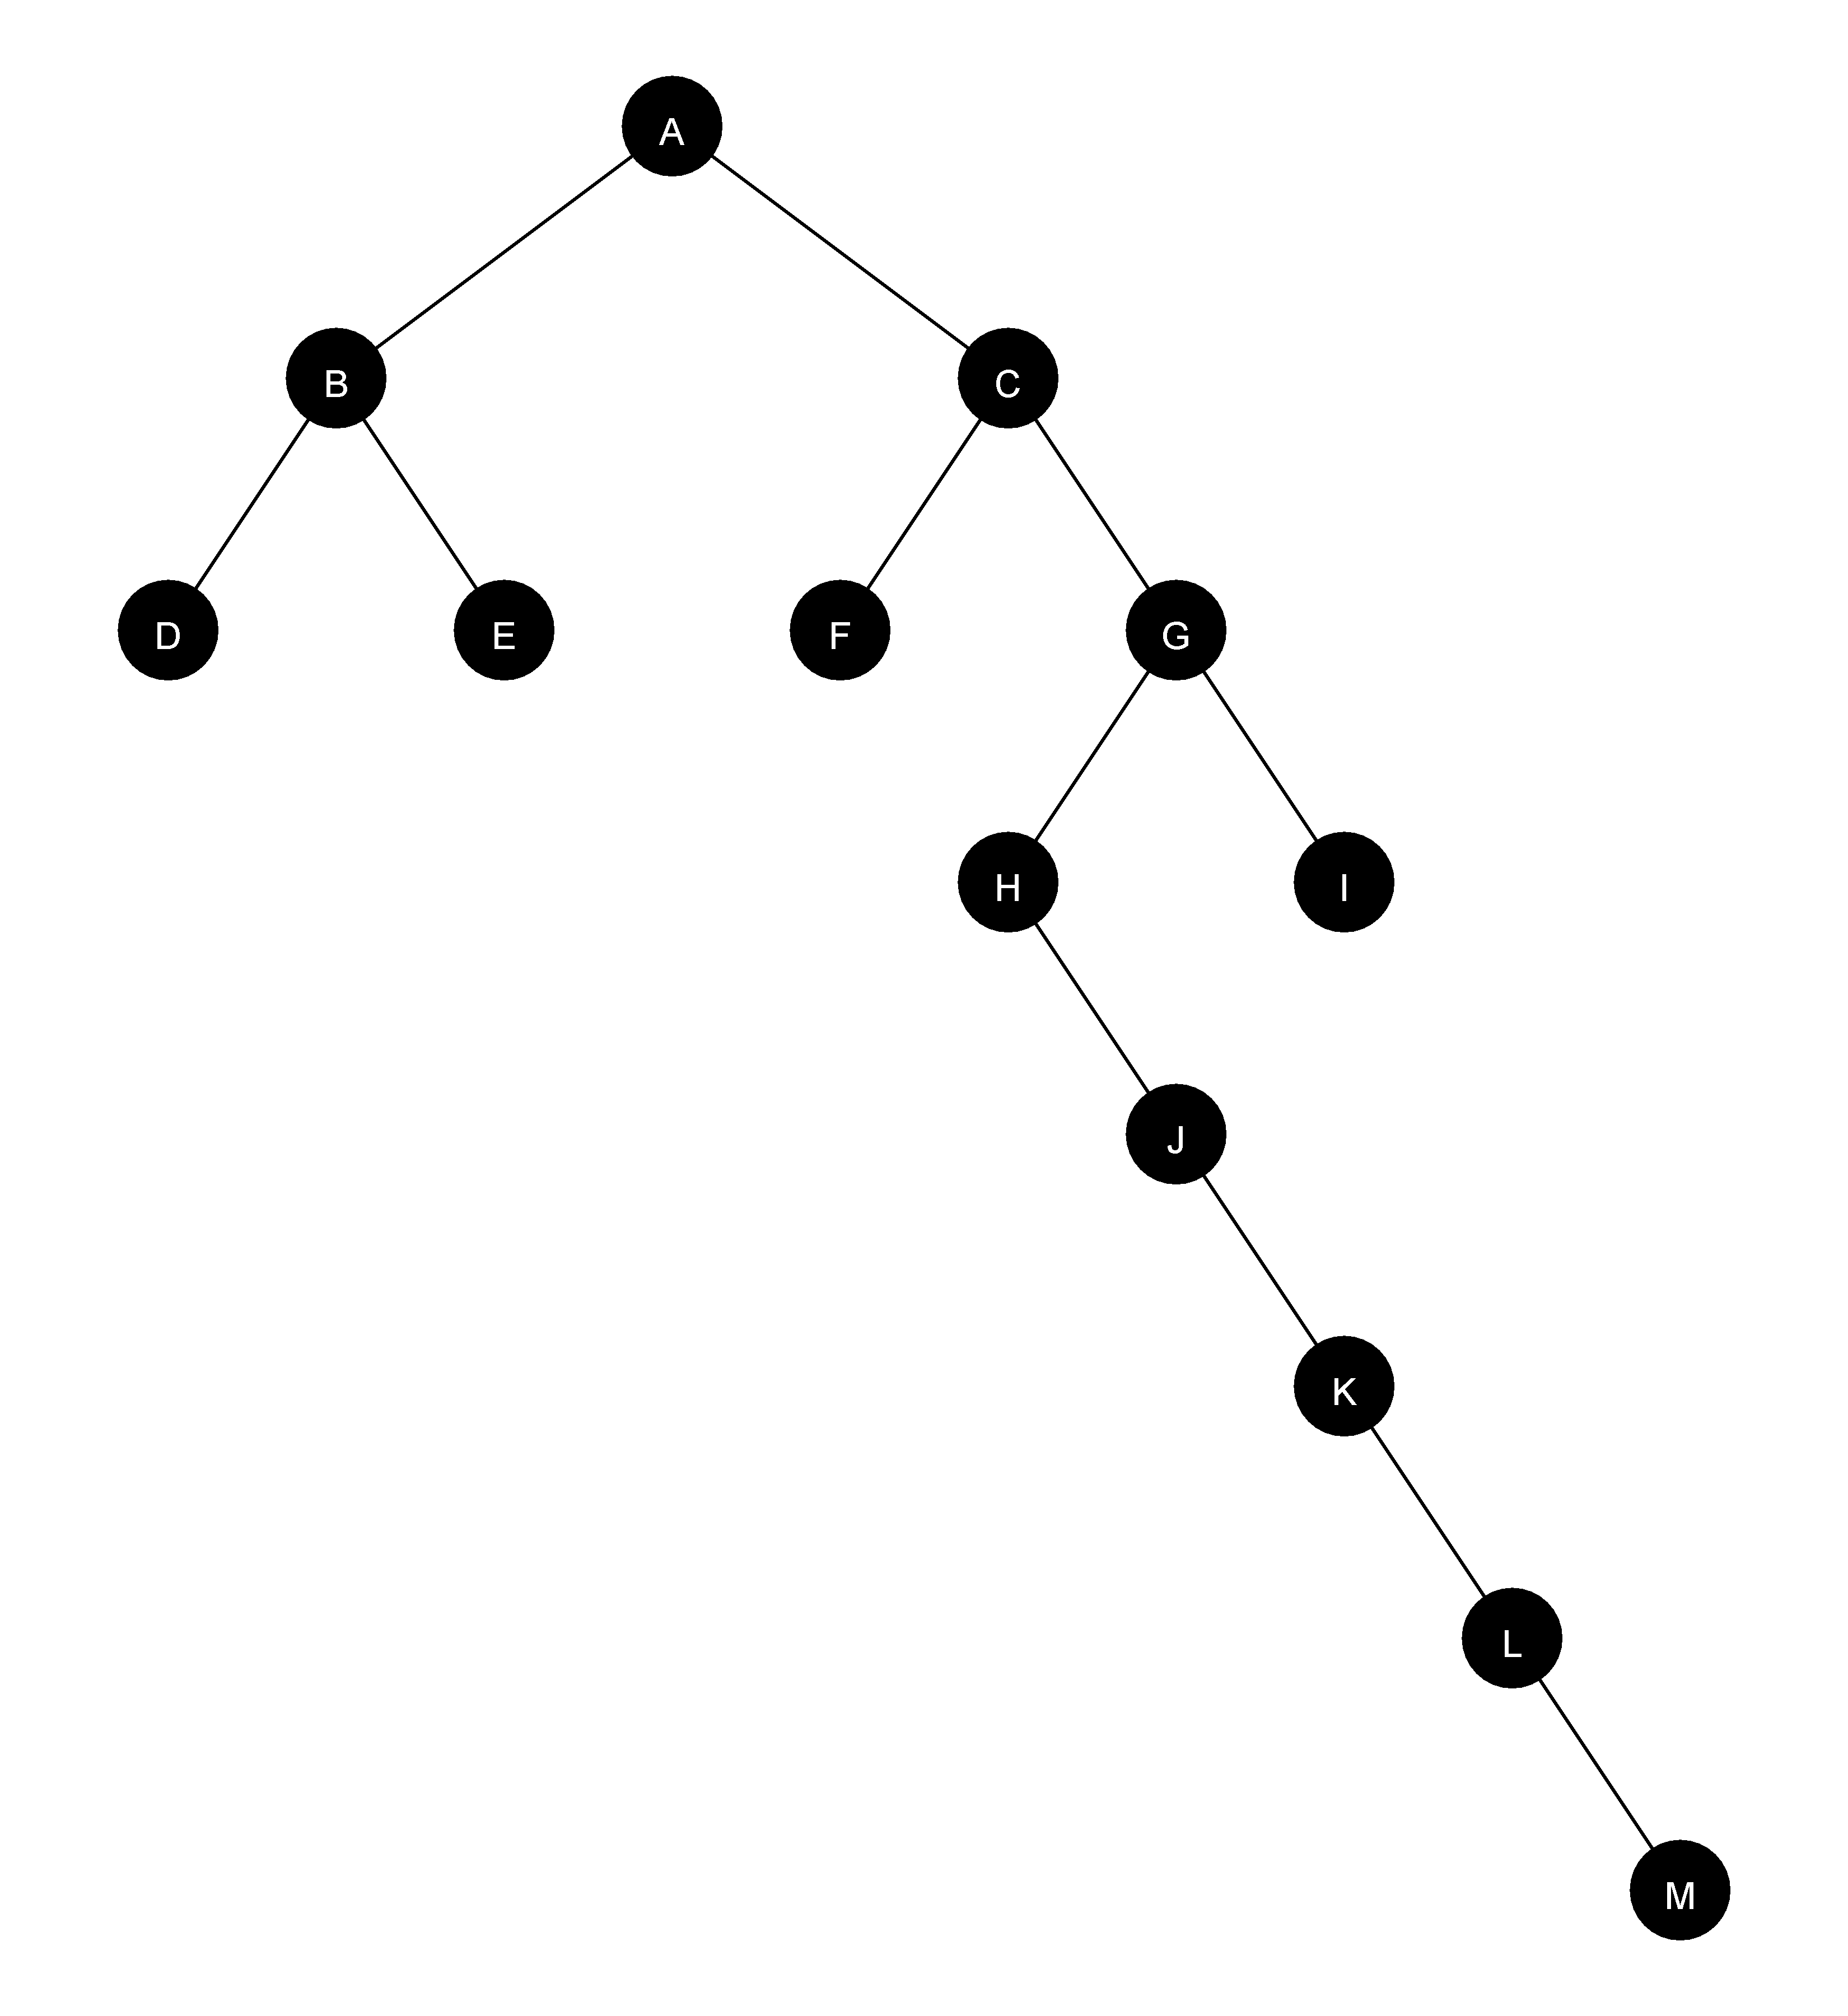
\includegraphics[scale = 0.05]{abbildungen/baum_algo_3_n1}
    \caption{Gezeichneter komplexer Baum durch den Tilford Algorithmus}
    \label{pic:baum_algo_3_n1} 
\end{figure}

\begin{figure}[H]
    \centering
    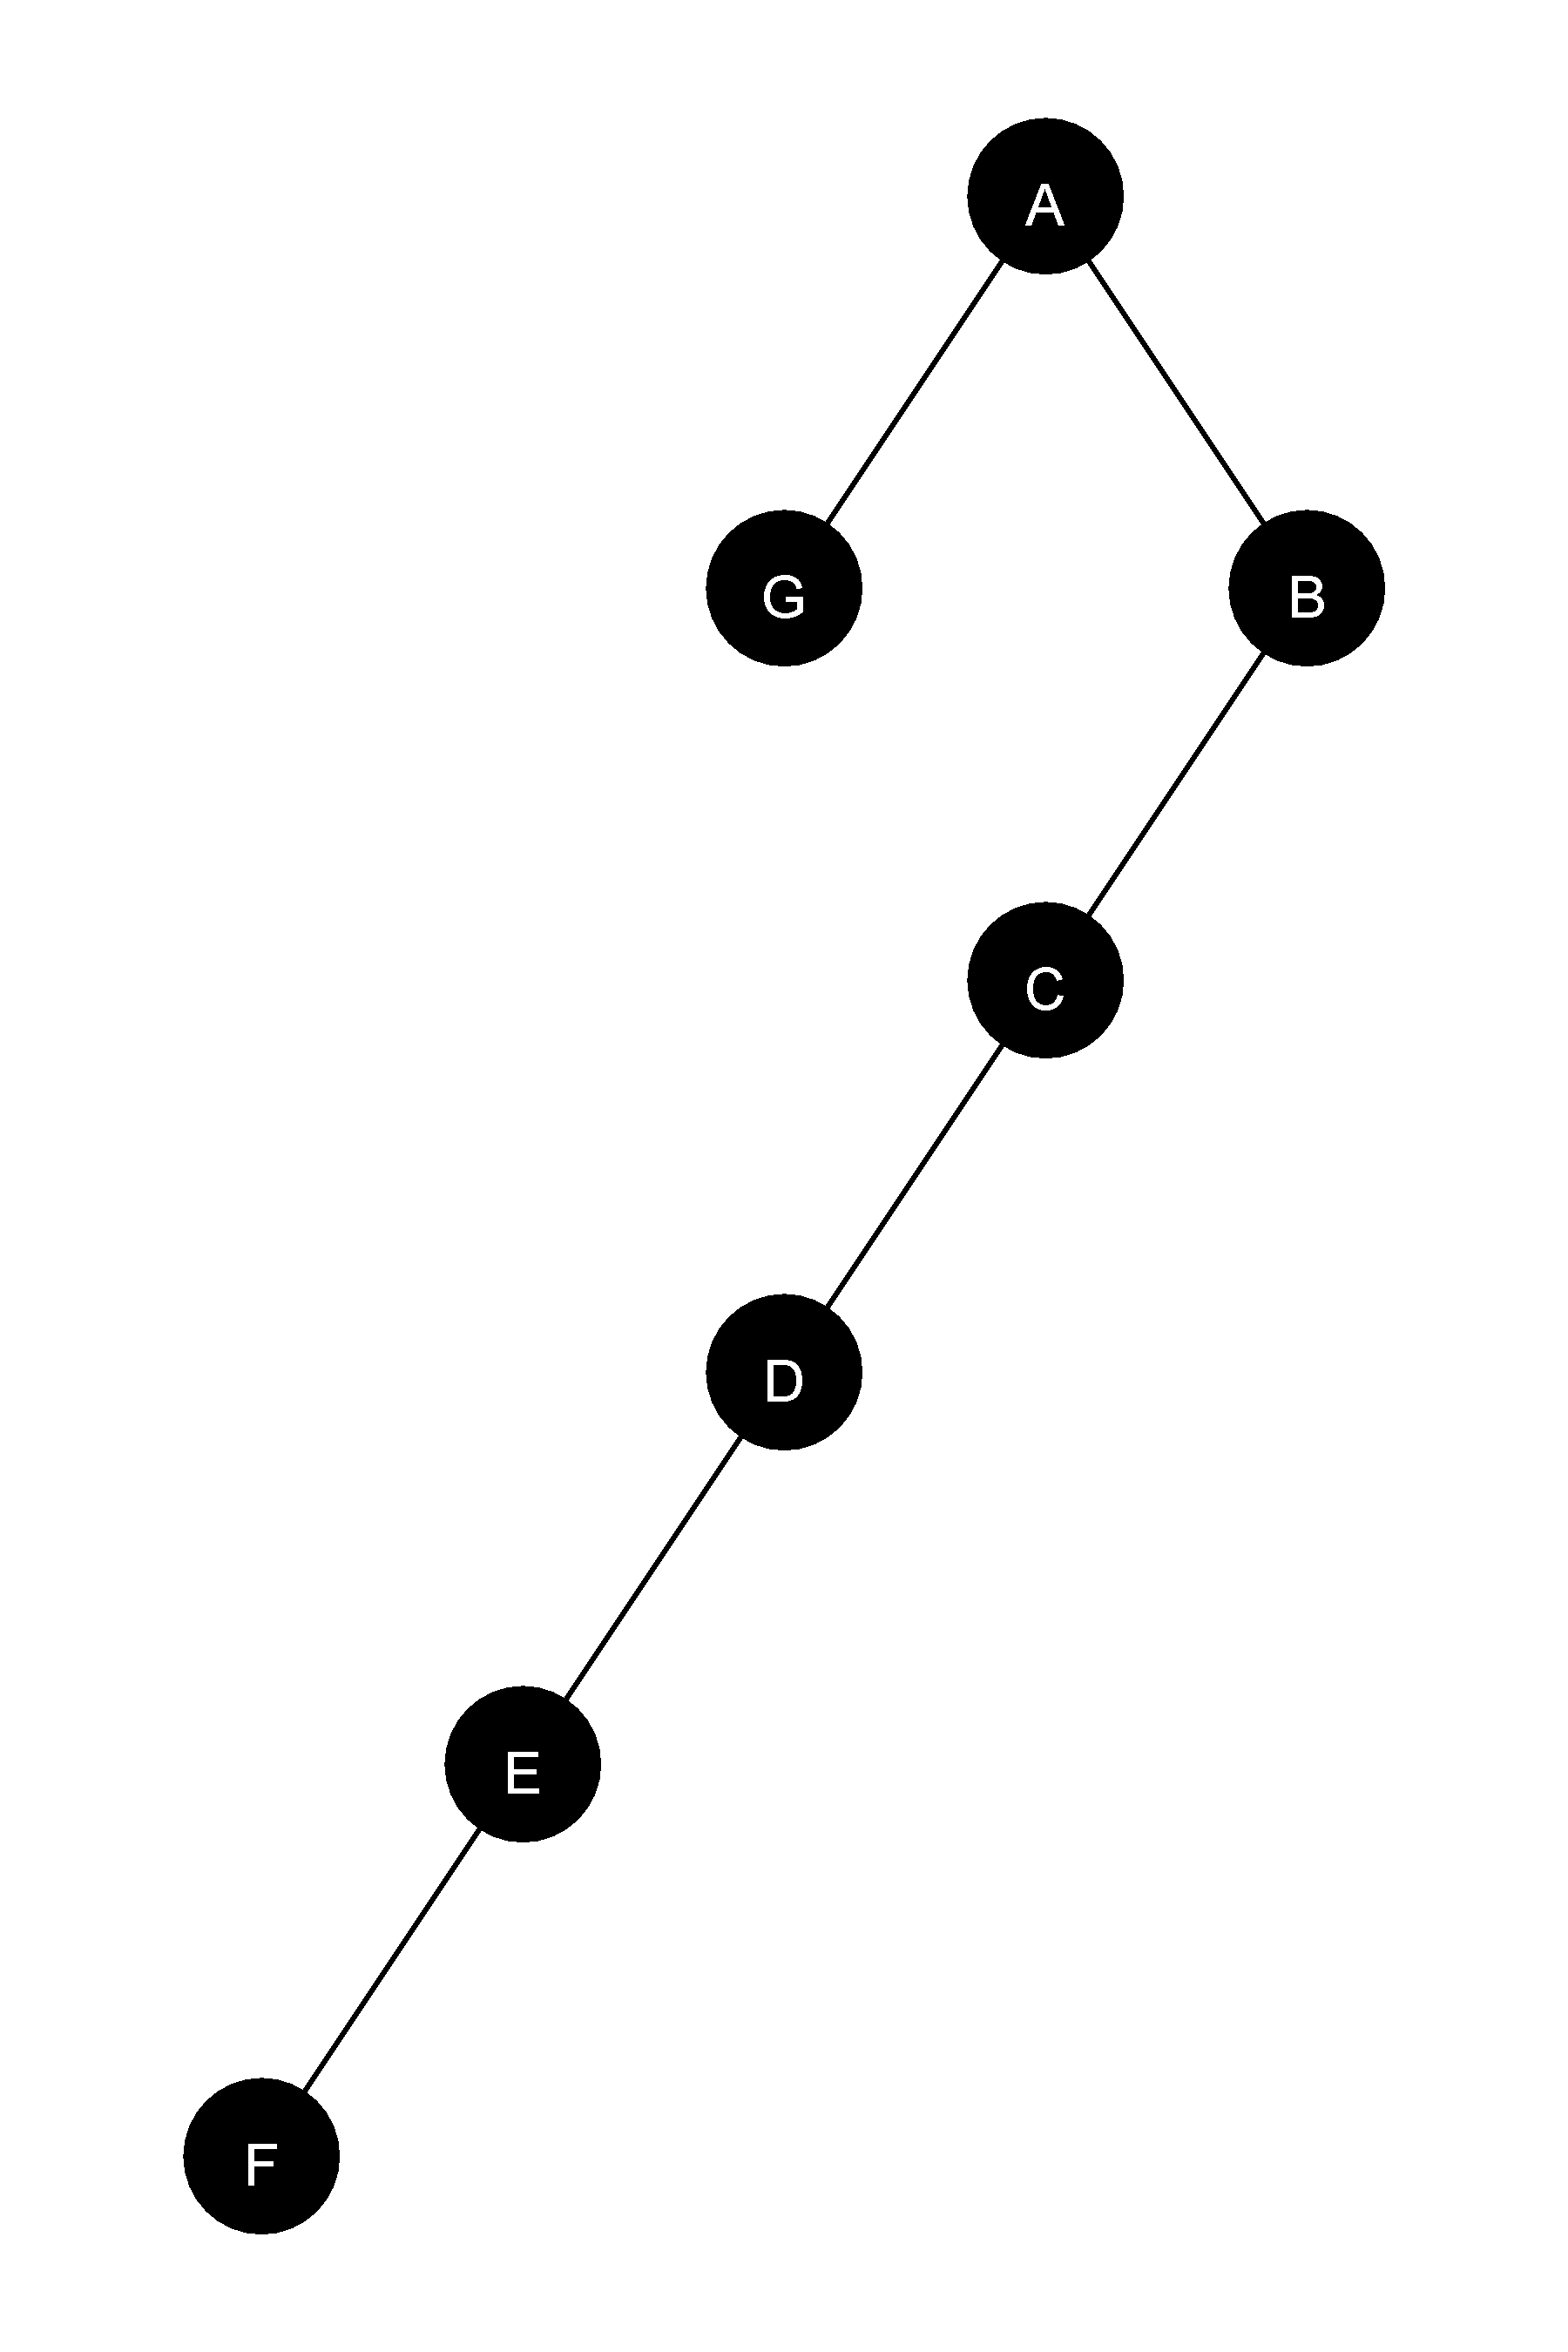
\includegraphics[scale = 0.07]{abbildungen/baum_algo_3_n2}
    \caption{Gezeichneter einfacher Baum durch den Tilford Algorithmus}
    \label{pic:baum_algo_3_n2} 
\end{figure}

Um diesen Algorithmus implementieren zu können, muss die zuvor erstellte BinaryKnoten-Klasse um ein 
Attribut erweitert werden: vom Typ Boolean mit dem Namen 'thread'. Zudem wurde eine weitere Klasse 
namens 'Extreme' definiert, die wie zuvor beschrieben, implementiert wurde. Die Extreme-Klasse sieht wie folgt aus:

\begin{figure}[H]
\begin{lstlisting}
private static class Extreme {
    BinaryKnoten knoten;
    int offset;
    int level;
    
    void set(BinaryKnoten k, int offset) {
        this.knoten = k;
        this.level = k.getHoehe();
        this.offset = offset;
    }
}
\end{lstlisting}
    \caption{Implementierung der Extreme-Klasse}
    \label{code:algo3_extreme}
\end{figure}

Ferner wurden die zuvor beschriebenen Prozeduren 'setup' und 'petrify' implementiert. Die implementierte Prozedur
'setup' unterscheidet sich zum zuvor beschriebenen Ablauf. Sie wird nun nicht mehr rekursiv aufgerufen und sie besitzt 
nur ein Eingabeparameter, den Wurzelknoten. Hiernach wird mithilfe der 'traversPostOrder'-Methode aus der 
BinaryKnoten-Klasse über den Baum traversiert.

\begin{figure}[H]
\begin{lstlisting}
public static void setup(BinaryKnoten wurzel) {
    // Initialisierungen von Variablen
    // <...>
    // Ueber den Baum in der Post-Order traversieren
    wurzel.traversPostOrder(k -> {
        BinaryKnoten knoten = (BinaryKnoten) k;

        // Bestimmen der Y-Koordinate
        knoten.setY(2 * knoten.getHoehe() + 1);

        // Vorlaeufige relative X-Koordinate bestimmem
        // <...>
    }
}
\end{lstlisting}
    \caption{Auschnitt aus der setup-Prozedur}
    \label{code:algo3_setup}
\end{figure}

Abweichend zum Ablauf entspricht die Y-Koordinate nicht der Höhe des Knotens. Stattdessen wird diese wie im 
Ablauf aus dem Kapitel \ref{chap:kapitel3_1_Ablauf} berechnet. Dies bietet den Vorteil, 
dass die Methodik zum Zeichnen der Bäume nicht verändert werden muss. Die weitere Implementierung folgt 
der Beschreibung aus dem Ablauf.

Die Implementierung der Prozedur 'petrify', entspricht der Beschreibung aus dem Ablauf.

Hiernach wurde die Prozedur 'algorithmus3' definiert. Diese ruft zu Beginn die beiden Prozeduren, 
'setup' und 'petrify' auf. Hiernach müssen die X-Koordinaten noch angepasst werden, da sich diese 
negativ sein können. Hierfür wird der kleinste X-Wert ermittelt, dessen absoluter Wert 
addiert mit eins in der Variable 'offset' gespeichert wird. Nun werden alle X-Koordinaten des 
Baums mit dem Wert aus 'offset' addiert. 

Zwei Beispielhafte Ergebnisse können in den Abbildungen \ref{pic:baum_algo_3_n1} 
und \ref{pic:baum_algo_3_n2} betrachtet werden.


\subsection{Vor- und Nachteile}

\subsection{Modifizierung des Algorithmus}